\documentclass[11pt]{article}
\usepackage{a3_report}
\usepackage{times}
\usepackage{url}
\usepackage{latexsym}
\usepackage{graphicx}
\usepackage{fancyhdr}

\pagestyle{fancy}
\fancyhead{}
\fancyfoot{}
\fancyfoot[C]{\thepage}

\aclfinalcopy % Uncomment this line for the final submission
%\def\aclpaperid{***} %  Enter the acl Paper ID here

\title{Stance detection}

\author{Romain THEODET \\
  {\tt theodet@student.chalmers.se}
}

\date{}

\begin{document}
\maketitle
\begin{abstract}
The goal of this paper is to implement a classifier that determines whether a given sentence
expresses a pro-vaccination or anti-vaccination point of view.
\end{abstract}

\section{Introduction}

Several solutions already exists to this problem ;
we will see in details the different models or pre-processing possible.
Then, with the processed data, which model to use, as again several model exist.

\section{Data}

In this section, we will focus on the data : how to get it, is it reliable,
and how to process it to remove possible junk.

\subsection{Dataset}

The dataset used has been built with tens of student from the YouTube comment section.

This dataset is fairly biased as it has been cherry-picked by the students in pro or anti-vaccination videos.
As such, the literacy level of the original authors might be biased,
since radical people are probably over-represented on the YouTube comment section,
We cannot then assume that our model would be able to understand more granular or grey-shaded stances,
especially from more educated or informed individuals.
This is especially true for the anti-vaccination community, which often writes "non visually appealing" comments.

Moreover, the data in itself isn't really reliable, albeit it has been reviewed by a pair.
The other students who classified the comments probably share common beliefs with the original student,
since we're all Master students in Computer Science living in a first-world  country. 
A third review could have helped to filter out even more ambiguous sentences.

To evaluate the quality of our model, we used separate training and test set.
Although it isn't a perfect solution, since the test set could be flawed and biased as well,
it is fairly easy to use and the results are straightforward.

\subsection{Pre-processing}

Our data, which is a string, has been processed to be represented as a matrix of words count.
This helps our model by only working on numeric values instead of characters.

The dataset has been unified to ASCII while keeping the case.
Some characters like double quotes or non-breaking spaces don't alter the stance in comparison of their ASCII equivalent,
but would induce some noise in the model.
Non-translatable characters like emojis have been simply removed.
This decision can be criticized, but with all the different encoding used by the students it could lead to unreadable characters.
This removal is only technical though, as emojis could certainly help the model in its stance detection,
like the needle or the red heart emoji.

We tried several pre-processing algorithm, if there was a conflict in the data row:

\begin{itemize}
\item Keep the majority, i.e. prioritize the most common opinion
\item Prioritize an anti-vaccine opinion, regardless of its distribution
\item Prioritize a pro-vaccine opinion
\end{itemize}

Each algorithm also exist in two variants : one who remove every row with some clear uncertainty ("-1" in the data),
and one less greedy where we try to ignore these red flags.
Around 9.7 \% of the data is marked as possibly uncertain, so it is not so trivial to remove this data,
since it still represent a fairly decent proportion of the full dataset.

The test set got the same pre-processing as the training set.

\section{Model}

Two models were tested, raising both slightly different results.
The models were chosen simply by testing all available models in \texttt{sklearn.feature\_extraction.text} . 

\subsection{HashingVectorizer}

This algorithm converts an array of strings to a matrix of token occurrences.
The matrix contains the word occurrence counts using hashing to differentiate words.

It has several advantages:
\begin{itemize}
\item It has a very low impact in memory, virtually null at initialization,
since the vocabulary is built dynamically
\item It can be partially fit or parallelized, as it holds no immutable state
\end{itemize}

There are several drawback, though:
\begin{itemize}
\item The transformation is one-way only, as there is no way to transform back the feature indice
to a string feature name, since it uses hash functions
\item If the hyperparameters are not well-chosen, collision between different words might happen
\end{itemize}

The two main hyperparameters are whether or not the strings should be case-sensitive,
and the number of features to keep.
To select this number of features, we tested several values and checked the resulting accuracy,
as it can be seen on Figure~\ref{fig:hash_accuracy}. We can see that the model converges
around $2^{18}$ features.

\begin{figure}[htb]
\begin{center}
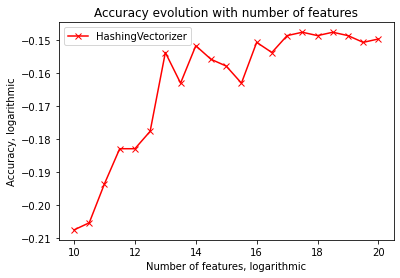
\includegraphics[width=70mm]{data/n_features_hash.png}
\end{center}
\caption{HashingVectorizer hyperparameter accuracy}
\label{fig:hash_accuracy}
\end{figure}

\subsection{TfidfVectorizer}

This algorithm convert the data to a matrix of TF-IDF (term frequency-inverse document frequency) features.
It is a numerical statistic that reflect how important a word is to the document.
To do so, this algorithm multiply two statistics, the term frequency and the inverse document frequency. 
The first one is the relative frequency of a word within the document,
while the second one is a measure of how much information the word provides, i.e. if it is common or rare across all documents.
Indeed, it seems obvious that the number of "the" in a message contains way less
information than the number of "sheep", which is not so common.

The main hyperparameters used here are, again, whether the words should be case-sensitive or not,
and bounds on the maximum and minimum frequencies.
It could be useful for some kind of data to filter out over-represented words, like "Subject" if we were working on e-mails,
or remove singular words like hash / GPG signatures / version numbers.
However, here the data is fairly concise, since we only kept the main content of the message.
As such, there isn't so much room to tweak these parameters.

\section{Results}

To evaluate the quality of our model, we simply measured its accuracy against the test set.
This might not be the perfect solution, but it is the easiest to implement and to interpret,
and doesn't require any additional processing.

We built several models on the dataset and compared their respective accuracy on table~\ref{table:model_accuracies}.
We also added a reference baseline, which simply randomly classify the data.

Since the baseline is around 50 \%, we can assume that the training set keeps the same proportion of pro and anti-vaccine comments.

With 1136 rows and 568 rows of each opinion, using a simple binomial distribution,
we can clearly say that any algorithm with a precision above 57.4 \% cannot be pure luck, as the standard deviation is 16.8.
This threshold correspond to the five-sigma, which says that there is
1 chance in 3.5 millions that this result would be only due to luck.

We calculated the accuracies of both models with all three data classification algorithms,
each with two binary parameters: whether or not filter out bad values, and if the words are case-sensitive.

Overall, we got 24 different accuracies for the different setups.

For all the tables~\ref{table:filter_accuracies},~\ref{table:case_accuracies},~\ref{table:preprocessing_accuracies} and~\ref{table:model_accuracies}, we took the average of all other configurations to avoid reporting biased data.

\begin{table}[htb]
\begin{center}
\begin{tabular}{l|l}
%\hline
\hline \bf Filtering mode & \bf Average accuracy in \% \\ \hline
Filter out uncertain & 86.39 \\
Keep uncertain & 86.76 %\\
%\hline
\end{tabular}
\end{center}
\caption{Effect of filtering on accuracy}
\label{table:filter_accuracies}
\end{table}

\begin{table}[htb]
\begin{center}
\begin{tabular}{l|l}
%\hline
\hline \bf Case sensitivity & \bf Average accuracy in \% \\ \hline
Case sensitive & 86.47 \\
All lowercase & 86.68 %\\
%\hline
\end{tabular}
\end{center}
\caption{Effect of case sensitivity on accuracy}
\label{table:case_accuracies}
\end{table}

\begin{table}[htb]
\begin{center}
\begin{tabular}{l|l}
%\hline
\hline \bf Preprocessing model & \bf Average accuracy in \% \\ \hline
Majority & 86.61 \\
Zeros prioritized & 86.66 \\
Ones prioritized & 86.46 %\\
%\hline
\end{tabular}
\end{center}
\caption{Accuracy depending of preprocessing}
\label{table:preprocessing_accuracies}
\end{table}

\begin{table}[htb]
\begin{center}
\begin{tabular}{l|l}
%\hline
\hline \bf Model & \bf Average accuracy in \% \\ \hline
Random & 50.00 (theoretical) \\
Tfidf & 86.69 \\
Hashing & 86.46 %\\
%\hline
\end{tabular}
\end{center}
\caption{Accuracy depending of model}
\label{table:model_accuracies}
\end{table}

Overall, the best model is actually the Tfidf one case insensitive
with the pro-vaccine stance prioritized while filtering confusing comments.\footnote
{According to the previous tables, it shouldn't be the most effective one,
but it actually is the best one from a really thin margin.}

With this model, we can see on Figure~\ref{fig:confusion} that there is almost the same amount of
false positives and false negatives.

\begin{figure}[htb]
\begin{center}
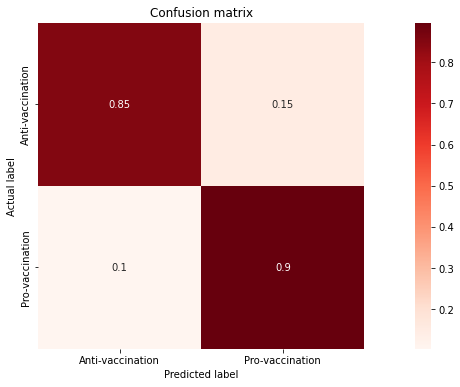
\includegraphics[width=70mm]{data/confusion.png}
\end{center}
\caption{Confusion matrix}
\label{fig:confusion}
\end{figure}

If we take some messages the model got wrong, we can actually see that some of them are clearly ambiguous.
For example, out of 10 comments, the following one were missclassified:

\begin{itemize}
\item\texttt{no other effective way}
\item\texttt{There also needs to be urgent outreach to young people saying” I don’t need the vaccine , I’m healthy You are healthy, until you aren’t}
\item\texttt{There should be more measures or schemes to improve our immune system rather than getting injections to prevent diseases.}
\item\texttt{the government explains the effectiveness of the vaccine}
\end{itemize}

Granted, there are also many counter examples where the message is clear, but a non-negligible part of the missclassified comments
are not so trivial.

With this \texttt{TfidfVectorizer}, we can extract the most important features in a comment.

For example, with the message "I think that the vaccine is a good idea. Vaccine helps people, and has been tested by doctors for years.",
the most important features are, in Table~\ref{table:feat_pro}:

\begin{table}[htb]
\begin{center}
\begin{tabular}{l|l}
%\hline
\hline \bf Word & \bf Score \\ \hline
helps & 0.39 \\
idea & 0.37 \\
doctors & 0.32 \\
tested & 0.31 \\
years & 0.26 %\\
%\hline
\end{tabular}
\end{center}
\caption{Features for a pro-vaccine comment}
\label{table:feat_pro}
\end{table}

However, with a clearly anti-vaccine stance like "Trump is right, vaccine cause autism. Do not listen to the doctors, you sheep. Jesus is watching you.",
the most important features are, in Table~\ref{table:feat_anti}:

\begin{table}[htb]
\begin{center}
\begin{tabular}{l|l}
%\hline
\hline \bf Word & \bf Score \\ \hline
watching & 0.33 \\
trump & 0.33 \\
jesus & 0.32 \\
autism & 0.32 \\
sheep & 0.32 %\\
%\hline
\end{tabular}
\end{center}
\caption{Features for an anti-vaccine comment}
\label{table:feat_anti}
\end{table}

These features scores make sense, as they correspond to "shock words", words quite rare in a text but full of meaning.
The best example would be "sheep", which strictly speaking only correspond to an animal, but helps the model to
classify a comment as anti-vaccine.
Same for the word "trump", which isn't even a word, but has correctly been associated with anti-vaccine speech.

\section{Conclusion}

Finally, our model works pretty well as is, and the preprocessing functions used seems to tend to nitpicking.

Such model could be used by FAANGs to automatically flag suspicious comments and prevent misconceptions about vaccines.

It should be noted, however, that this kind of algorithm is obviously clearly oriented in the way the dataset is oriented ;
a bad actor could train such model to flag some less obvious features like race or sex.

\bibliographystyle{a3_report}
\bibliography{template}

\end{document}
